\section{Simulation}
\label{sec:sim}

To investigate the performance of the trigger under HL-LHC conditions, we developed HOTPOT, a standalone simulation of the MMTP trigger in C++. We simulate downward moving cosmic tracks, with a variable rate of background, in a rectangular region of the MM detector. We look at two lengths of strips: 2.2 m and 0.5 m, which should capture the trigger performance at the top of LM2 and the bottom of SM1. The output of the simulation is a collection of possible triggers found by the MMTP. For each event, we generate one downward muon track, and then add background hits in a window 40 BCs wide, where the first background hit comes 16 BCs before the first muon hit.
\par We aim to be as faithful and complete as possible. To consider several upstream electronics effects, some of which are not considered in the current ATHENA simulation, we ``feed" the cosmic track hits and background hits through the VMM and the ADDC. This includes the 8-ART signal per BC processing limit of the ADDC and the 1-ART signal per BC limit of the VMM. The position of the cosmic muon hit is also smeared with a gaussian with a $\sigma$ of 1 strip. This is motivated by our previous trigger data, described in \cite{mmtp}. Fig. \ref{fig:art_xres} shows the position resolution of the ART. The RMS of the distribution is about 0.5 mm, or approximately the strip pitch. The timing of the hit is smeared with a gaussian with a $\sigma$ of 32 ns to simulate the ART time resolution measured in \cite{mmtp}.
\begin{figure}[!htpb]
  \begin{center}
    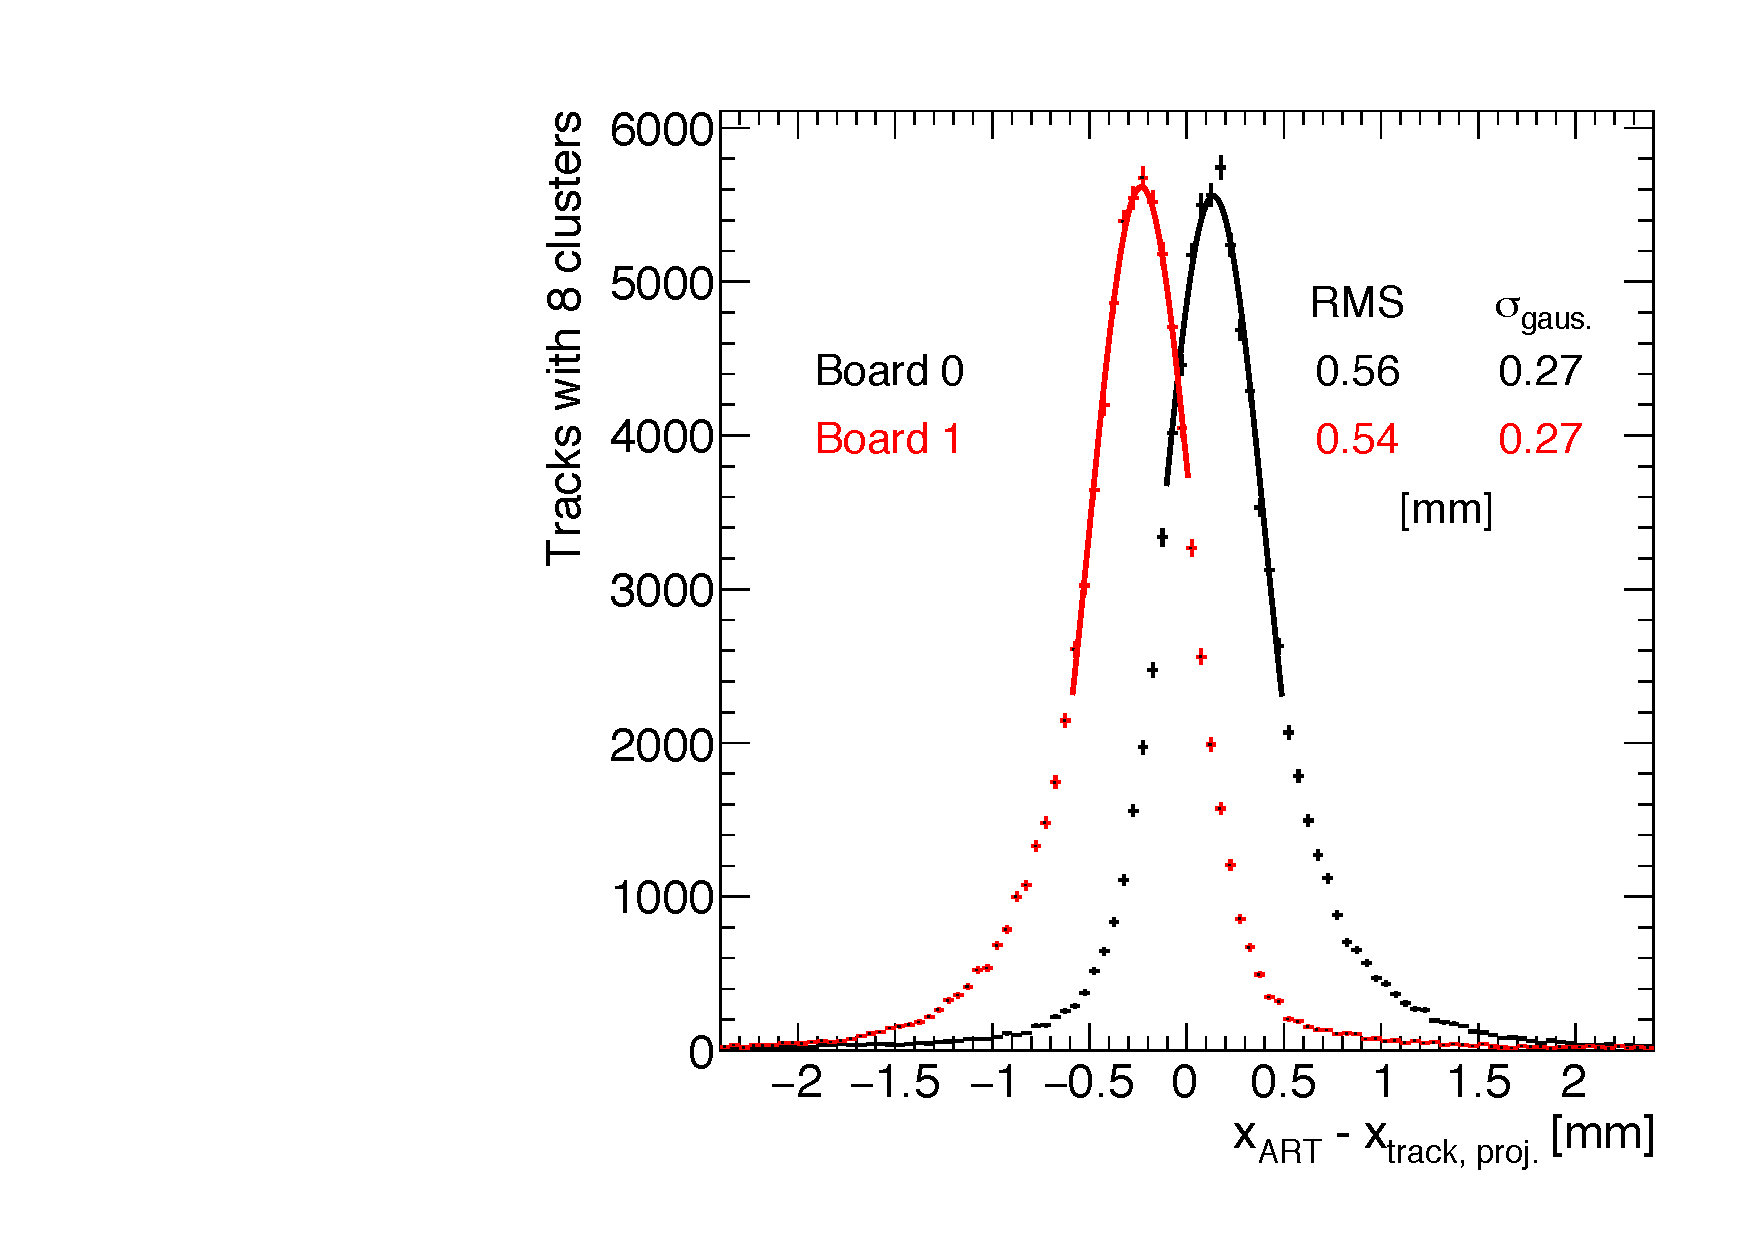
\includegraphics[width=0.48\textwidth]{figures/xres_art_boards01.pdf}
    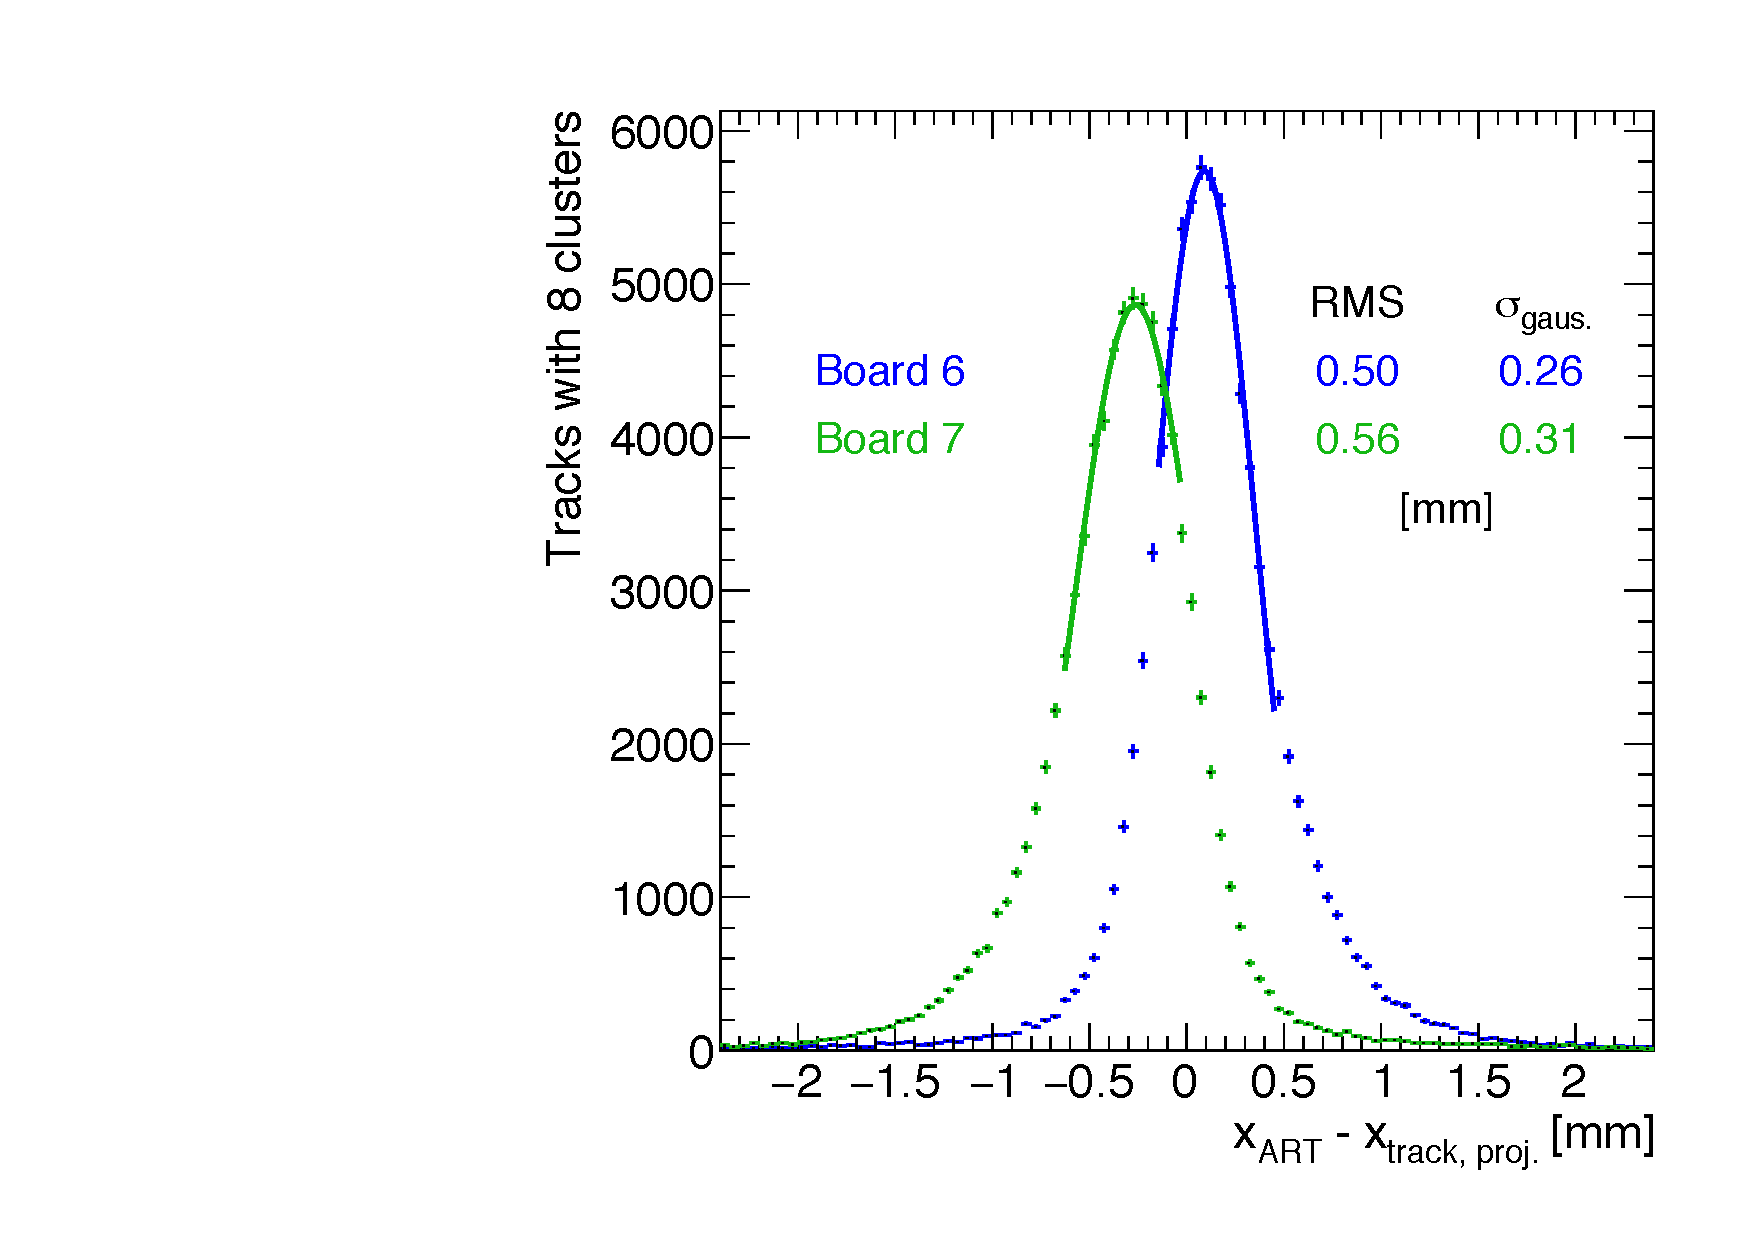
\includegraphics[width=0.48\textwidth]{figures/xres_art_boards67.pdf}
  \end{center}
  \vspace{-10pt}
  \caption{The x-residuals (precision coordinate) of the ART hit compared to the projected x-position using a track fit to 8 MMFE8 clusters, for each of the $X$ boards, indexed 0 \& 1 (left), 6 \& 7 (left).}
  \label{fig:art_xres}
\end{figure}

\par 
We then feed the ART hits through an implementation of the MMTP algorithm. The algorithm has two versions: the nominal (original) algorithm, and the proposed algorithm, described in Sections \ref{sec:nominal} and \ref{sec:stereoroads}, respectively. The algorithm collects ART hits over a fixed time collection window (8 BCs), looks for and then outputs candidate triggers. Since the interface with the sTGC detectors and Sector Logic has yet to be determined, we study the resolution by ordering the output triggers by how many hits they contain from the original muon track (dubbed ``real muon hits"). We then randomly choose one of the triggers with the maximum number of real muon hits.
There are several tunable parameters that are affect the MMTP performance. The list of parameters and their default values are given in the following table:
\begin{center}
\begin{tabular}{ |c|c| } 
 \hline
 \textbf{Parameter} & \textbf{Default Value} \\ 
 MM chamber efficiency & 100\%  \\ 
 ART time resolution (ns) & 32 \\ 
 ART time collection window (BC) & 8 \\ 
 Nominal road size (strips) & 8 \\
 ART position resolution (strips) & 1\\
 Trigger plane coincidence requirement & 3X3UV \\
 Uncorrelated background rate (kHz) per strip & 40\\
 Region size (roads) & 2.2 m strips: 136, 0.5 m strips: 96\\
 \hline
\end{tabular}
\end{center}
